\documentclass[a4paper,12pt]{article}
\usepackage{geometry}
\usepackage{amsmath}
\usepackage{graphicx}
\usepackage{fancyhdr}
\usepackage{titlesec}
\usepackage{setspace}

\usepackage{siunitx}
\usepackage{subcaption}
\usepackage{flafter}
\usepackage{float}
\usepackage{tabularx}
\usepackage{amsfonts}
\usepackage{placeins}
\usepackage[utf8]{inputenc}\usepackage[
    backend=biber,
    style=numeric,
    sorting=none
    ]{biblatex}

\addbibresource{mybibliography.bib}
\doublespacing{}
% Adjust page margins
\geometry{left=2.0cm,right=2.0cm,top=2.0cm,bottom=2.0cm}

% Set up header and footer
%\pagestyle{fancy}
%\fancyhf{}
%\rhead{\thepage}
%\lhead{\textit{Mathematics Internal Assessment}}
%\renewcommand{\headrulewidth}{0.4pt}

% Customize section and subsection formatting
\titleformat{\section}{\normalfont\Large\bfseries}{\thesection}{1em}{}
\titleformat{\subsection}{\normalfont\large\bfseries}{\thesubsection}{1em}{}
\titleformat{\subsubsection}{\normalfont\normalsize\bfseries}{\thesubsubsection}{1em}{}

\begin{document}

\title{\textbf{Mathematics AA HL Internal Assessment}\\\large Exploration: The mathematics behind locating a lost phone.}
\author{~}
\date{~}
\maketitle

\newpage
\section{Introduction}
Within an area an electromagnetic waves emitting device, such as a mobile phone, is situated at an unknown location. However, there are 3 base stations, placed at a known distance away from each other. 
These base station receive the EM radiation from the phone. The role of these base stations, is to measure the intensity of the EM wave received. This mathematical exploration aims to find the position of the phone relative to one of the base stations, using the distances between each base station, and the ratio of the intensity of the EM wave the base stations receive.
\\\\
Let the EM waves transmitting device be denoted as $P$ at position $(P_x, P_y)$. Let the three base stations be denoted as $B_0$, $B_1$ and, $B_2$. The intensities received from them are $I_0$, $I_1$ and, $I_2$ respectively. If $B_0$ is located at position $0,0$, then $B_1$ is located at $(0,L_1)$ and $B_2$ at $(x_2,y_2)$, such that, $x_2 \mathbb{R}-0, y_2\in \mathbb{R}$ and $B_2$ is distance $L_2$ from $B_0$.
They are set up in a way, such that $B_0$, $B_1$ and $B_2$ are noncollinear. Using the known ratio of intensities $k_1=I_0:I_1$ and $k_2=I_0:I_2$, this exploration aims to determine $(P_x, P_y)$, where $k_1,k_2>0$
\subsection{ Background Knowledge}
% Provide necessary mathematical background
\textbf{Intensity of light:} The EM wave transmitting device transmits EM waves uniformally in all direction following the inverse square law, which states that the strength of the wave is proportional to $\frac{1}{d^2}$, where $d$ is the distance from transmitter. 
The formula for intensity of light, which can be measured by the base stations is, $I=\frac{P_w}{4\pi d^2}$, where $P_w$ is the power of the EM wave transmitted from the GPS device, 
and $d$ is the distance between point of measurement of intensity and source (phone)~\cite{2}
\\
For example, if the Power of the EM wave is given to be $P_w=1600W$ and $B_0$ measures an intensity of $I_0=100W/m^2$, then the distance between $B_0$ and $P$ is 
\begin{equation*}
    d=\sqrt{\frac{1600W}{100\frac{W}{m^2}4\pi}}= \frac{2}{\sqrt{\pi}}= 1.12837\dots m\approx 1.13m
\end{equation*}
Hence, in this example, the device is about $1.13m$ away from the base station. Since, $d$ is a scalar not a vector, the direction of $d$ is unknown. With a fixed value $1.13 m$, $P$ lies on a circle with the radius $1.13 m$ and centered at $B_0$.
\\
Therefore, it is also important to know the conditions under which of a 2 variable quadratic equation takes form of a circle.
\\\\
\textbf{Properties of quadratic equations with 2 variables:} If an equation is in the form of $Ax^2 +Bxy +Cy^2 +Dx +Ey +F = 0$, and $B^2-4AC<0$~\cite{1}, the function is a circle or an ellipse. Additionally, this equation is a function of a circle under the conditions that $A>0, B=0, C=A$ 
For example, the is quadratic equation: $0.7x^2 0xy +0.7y^2 + 6.8x - 1.1y + 7.3 = 0$, is in the general form of a 2 variable quadratic equation, where:
\begin{equation*}
    \begin{split}
        A&=0.7,~B=0\\
        C&=0.7,~D=6.8\\
        E&=-1.1,~F=7.3\\
    \end{split}
\end{equation*}
Here, $B^2-4AC=-1.96<0$, and $A=0.7>0, B=0, C=A$. Hence, the plot of this function (\textit{see Figure~\ref{fig:abc}}) is a circle or ellipse:
\begin{figure}[H]
    \caption{The graph of the 2 variable quadratic from the example}
    \centering 
    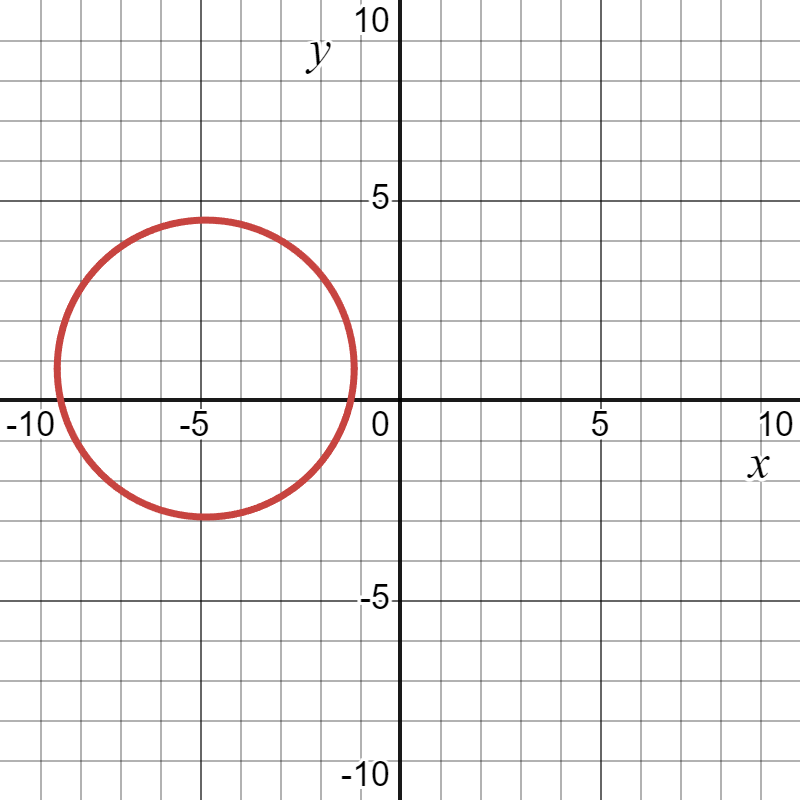
\includegraphics[width=0.5\textwidth]{abc.png}
~\label{fig:abc}
\end{figure}






Let $I_0$ and 




\section{Solution}
\subsection{Solution on 1 Dimensional Case}

Firstly, a 1 dimensional case is considered where, only the base stations $B_0$ and $B_1$ with the distance between them being $L_1$,  are considered. The phone $P$, located at $P_y$, has can move between the two base stations. 
\begin{figure}[H]
    \caption{Experimental setup for 2 sources with GPS device moving only vertically}
    \centering 
    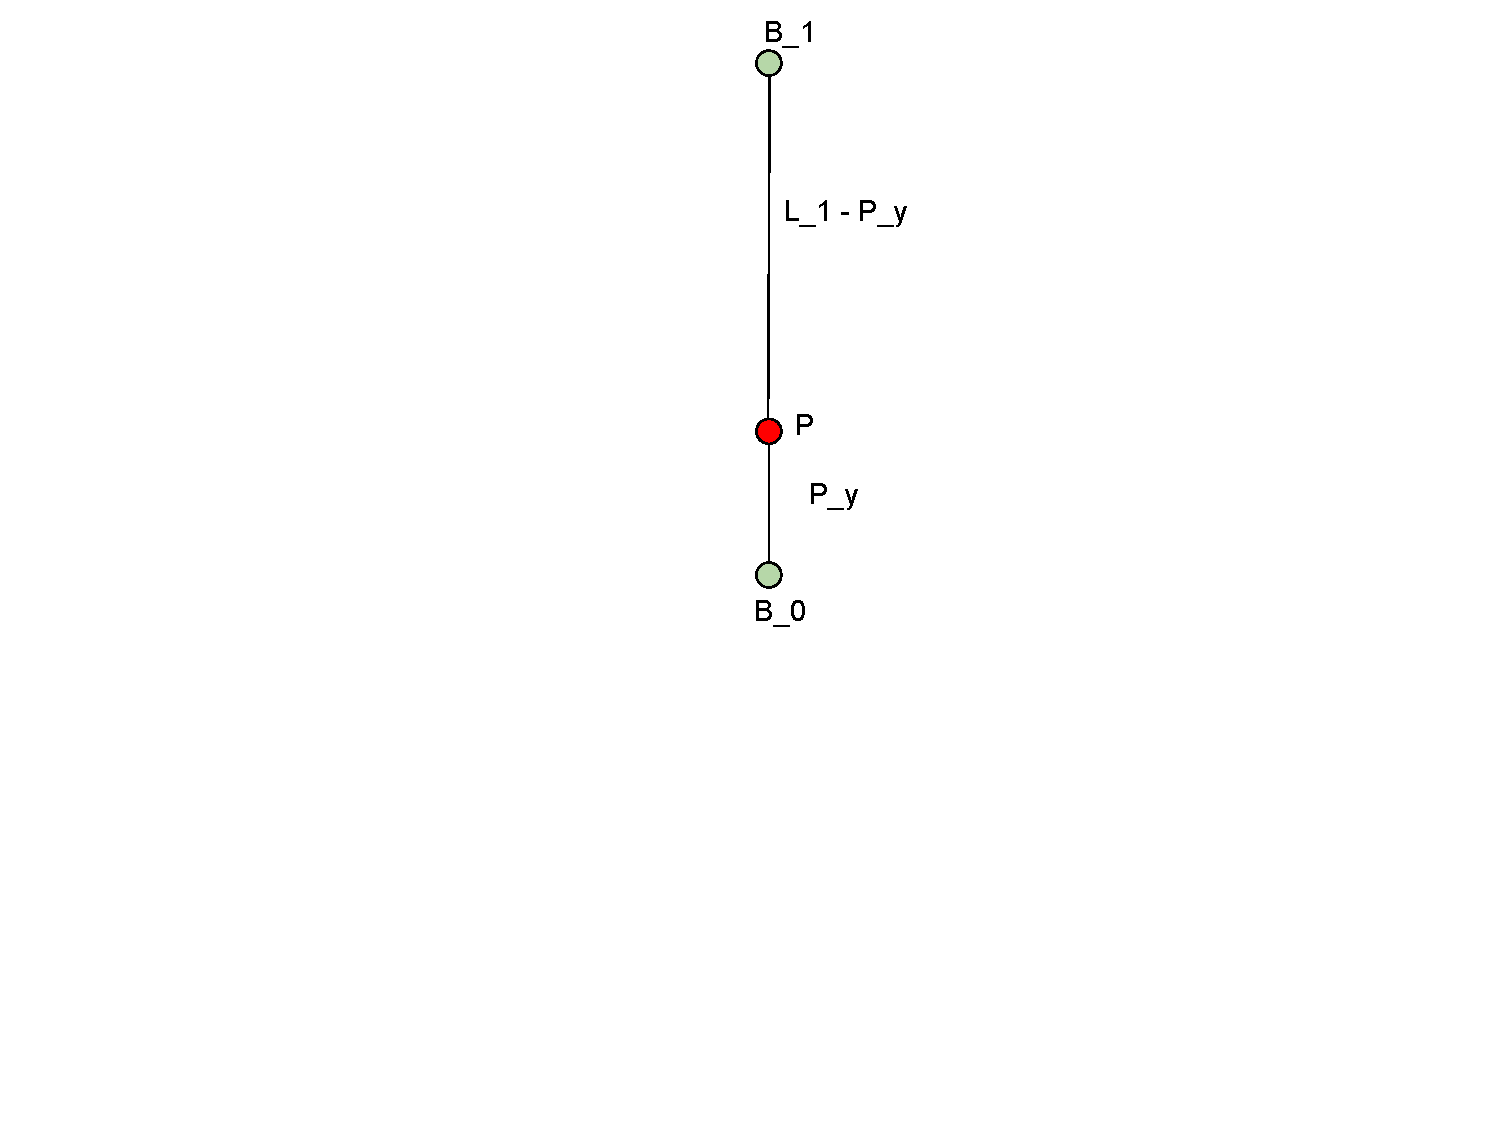
\includegraphics[width=0.7\textwidth]{draw1.pdf}
~\label{fig:draw1}
\end{figure}

$I_0$ and $I_1$ are the intensities of EM waves received at $B_0$ and $B_1$ respectively. Let, $k_1$ be the ratio of $I_0:I_1$. The EM wave at source has a power of $P_w [W]$.
\\
Using the equation of Intensity, $I_0=\frac{P_w}{4\pi P_y^2}$ and $I_1=\frac{P_w}{4\pi (L_1-P-y)^2}$.
Hence, 
\begin{equation*}
    \begin{split}
    k_1 &= \frac{I_0}{I_1}=\frac{P_w}{4\pi P_y^2}\cdot\frac{4\pi (L_1-P-y)^2}{P_w}\\\\
    k_1 &= \left(\frac{L_1-P_y}{P_y^2}\right)^2=\left(\frac{L_1}{P_y}-1\right)^2\\
    \end{split}
\end{equation*}
\begin{equation}
    P_y = \frac{L_1}{\sqrt{k_1}+1}
\label{eq:1d_sol}
\end{equation}
Hence, knowing the ratio of intensities received between the two sources, on a 1 dimensional line such that $B_0$,$B_1$ and $P$ are collinear, the location of $P$ is $P_y=\frac{L_1}{\sqrt{k_1}+1}$.


\subsection{Solution on a 2D area}
In the 1 Dimensional case, the location of $P$ was defined by $P_y$, as there was only one degree of freedom. In a 2 dimensional case, the location of $P$ is defined by $(P_x, and P_y)$.

\begin{figure}[H]
    \caption{Experimental setup for 2 base stations with the Phone having 2 degrees of freedom (x-axis and y-axis)}
    \centering 
    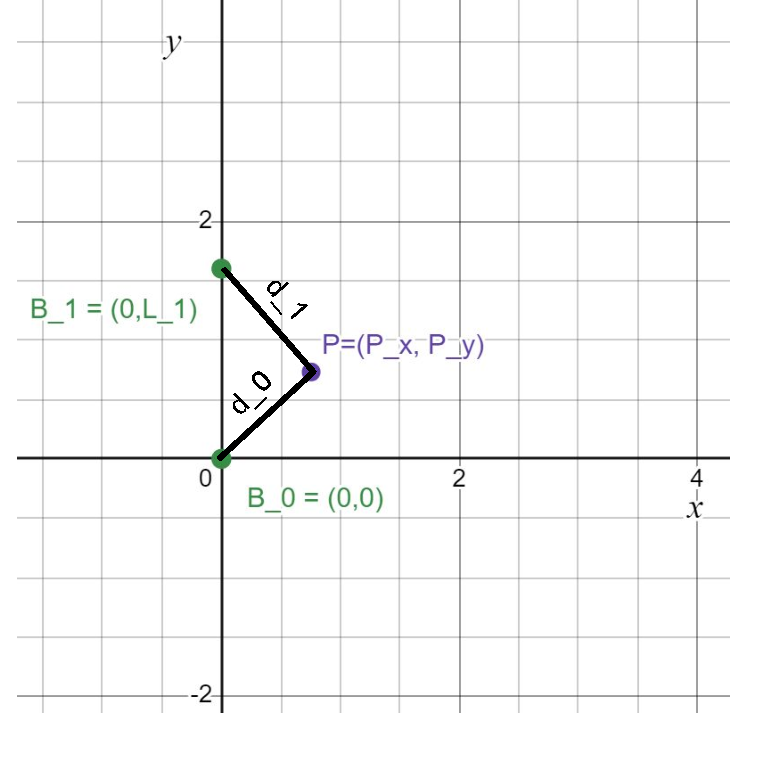
\includegraphics[width=0.7\textwidth]{draw2.pdf}
~\label{fig:draw2}
\end{figure}
The point or phone's location, $P$ is unknown. However, the distance between a base station and $P$ can be calculated using the Pythagoras theorem. The distance between $B_0$ and $P$ is $d_0=\sqrt{P_y^2 + P_x^2}$
and with $B_1$, $d_1=\sqrt{(L_1-P_y)^2 + P_x^2}$.

Trying to find the equation of $k_1$, with $d_0$ and $d_1$, gives:
\begin{equation*}
    \begin{split}
        k_1 &= \frac{I_0}{I_1}=\frac{P_w}{4\pi d_0^2}\cdot\frac{4\pi d_1^2}{P_w}\\
        k_1 &= \frac{I_0}{I_1}=\frac{P_w}{4\pi \sqrt{P_y^2+P_x}^2}\cdot\frac{4\pi \sqrt{(L_1-P_y)^2 +P_x^2}^2}{P_w}\\
    \end{split}
\end{equation*}
Simplifying this equation gives:
\begin{equation*}
    \begin{split}
    k_1 &= \frac{(L_1-P_y)^2 + P_x^2}{P_x^2 + P_y^2}\\
    k_1 &(P_x^2 + P_y^2) = (L_1-P_y)^2 + P_x^2\\
    P_x^2 & (k_1-1)  = (L_1-P_y)^2 - k_1P_y^2 = L_1^2 +2L_1P_y^2 -P_y^2(k-1)
    \end{split}
\end{equation*}
This equation can be rearranged to:
\begin{equation}
    (k_1-1)P_x^2 + (k_1-1)P_y^2 +2L_1P_y -L_1^2 =0\
\label{eq:circ1gen}
\end{equation}
The~\textit{equation~\ref{eq:circ1gen}}, can be arranged in the form $Ax^2 +Bxy +Cy^2 +Dx +Ey +F = 0$, where
\begin{equation*}
    \begin{split}
        A&=(k_1-1),~B=0\\
        C&=(k_1-1),~D=0\\
        E&=2L_1,~F=-L_1^2\\
    \end{split}
\end{equation*}
This gives 3 cases, depending on the value of $k_1$.
\textbf{Case 1: $k_1>1$}\\
In this case, the conditions for the equation forming a circle are satisfied as $A>0, B=0, C=A$.  Hence, this equation can be converted to a standard form equation of a circle, to find its center and radius.
\begin{equation*}
    \begin{split}
        &(k_1-1)P_x^2 + (k_1-1)P_y^2 +2L_1P_y = L_1^2\\\\
        &(k_1-1)\left(P_x^2 + P_y^2 + \frac{2L}{k_1}P_y\right)=L_1^2\\\\
        &P_x^2 + \left(P_y+ \frac{L_1}{k_1-1} \right)^2 - \left(\frac{L_1}{k_1-1}\right)^2 = \frac{L_1^2}{k_1-1}\\\\
        &P_x^2 + \left(P_y - \frac{-L_1}{k_1-1} \right)^2 = \frac{L_1^2}{(k_1-1)} + \frac{L_1^2}{(k_1-1)^2}\\\\
        &P_x^2 + \left(P_y - \frac{-L_1}{k_1-1} \right)^2 = \frac{L_1^2\cdot (k_1-1)}{(k_1-1)\cdot (k_1-1)} + \frac{L_1^2}{(k_1-1)^2}\\\\
        &P_x^2 + \left(P_y - \frac{-L_1}{k_1-1} \right)^2 = \frac{L_1^2(k_1)}{(k_1-1)^2}\\\\
    \end{split}
\end{equation*}
\begin{equation}
    C_1: P_x^2 + \left(P_y - \frac{-L_1}{k_1-1} \right)^2 = \left(\frac{L_1}{k_1-1}\sqrt{k_1}\right)^2
\label{eq:circ1sta}
\end{equation}
This shows that, knowing the ratio of intensities from 2 base stations the possible coordinate of $P$ for the circle $C_1$ seen in~\textit{equation~\ref{eq:circ1sta}}, 
which is centered at $(0,\frac{-L_1}{k_1-1})$ and has a radius $R_0=\frac{L_1}{k_1-1}\sqrt{k_1}$ and is a distance $S_{c1}=\frac{-L_1}{k_1-1}$ units away from $B_0$.
It should also be noted, that the center of $C_1$ lies on the same line $M_1: x=0$ that passes through $B_0$ and $B_1$.
\\
\textbf{Case 2: $k_1=1$}\\
In such a case, $A=0, B=0, C=0, D=0$. Hence, the~\textit{equation~\ref{eq:circ1gen}}, simplifies to 
\begin{equation*}
    \begin{split}
        &0x^2 + 0xy + 0y^2 + 0x + 2L_1y - L_1^2 = 0\\
        &y=\frac{L_1^2}{2L_1}=\frac{L_1}{2}
    \end{split}
\end{equation*}
As this equation is an equation of a horizontal line $T_1$, the infinitely many possible positions of $P$ are $(P_x, P_y)=(x, \frac{L_1}{2})$, where $x,L_1\in \mathbb{R}$. 
\\
\textbf{Case 3: $0<k_1<1$}\\
In such cases, instead of defining $k_1$ as the ratio of $I_0:I_1$ it can be defined as $I_1:I_0$, which would lead to the first case, where the possible positions of $P$ form a circle with~\textit{equation~\ref{eq:circ1sta}}. 
Hence, this case can be disregarded as it has the same effect as~\textbf{Case 1}.
\\\\
Taking into account the 3rd base station, this procedure can be repeated using the ratio $k_2=I_0:I_1$. Here, $B_1$ is disregarded and instead $B_2$ is used. The~\textit{Figure~\ref{fig:draw3_1}}, shows the base stations taken into account when calculating $C_1$, and~\textit{Figure~\ref{fig:draw3_2}},
shows the base stations this procedure is extended to. 
\begin{figure}[!ht]
    \centering
    \begin{minipage}{.5\textwidth}
      \centering
      \captionof{figure}{}
      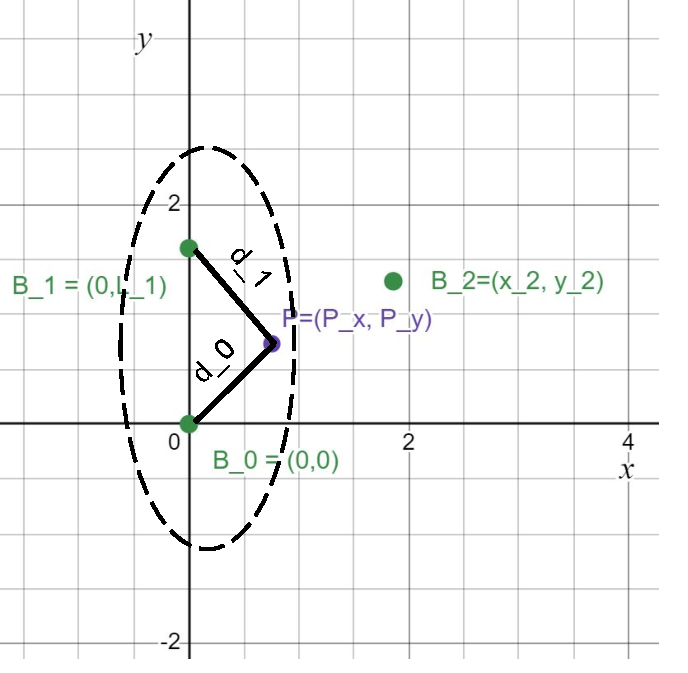
\includegraphics[width=\linewidth]{draw3.1.pdf}
~\label{fig:draw3_1}
    \end{minipage}%
    \begin{minipage}{.5\textwidth}
      \centering
      \captionof{figure}{}
      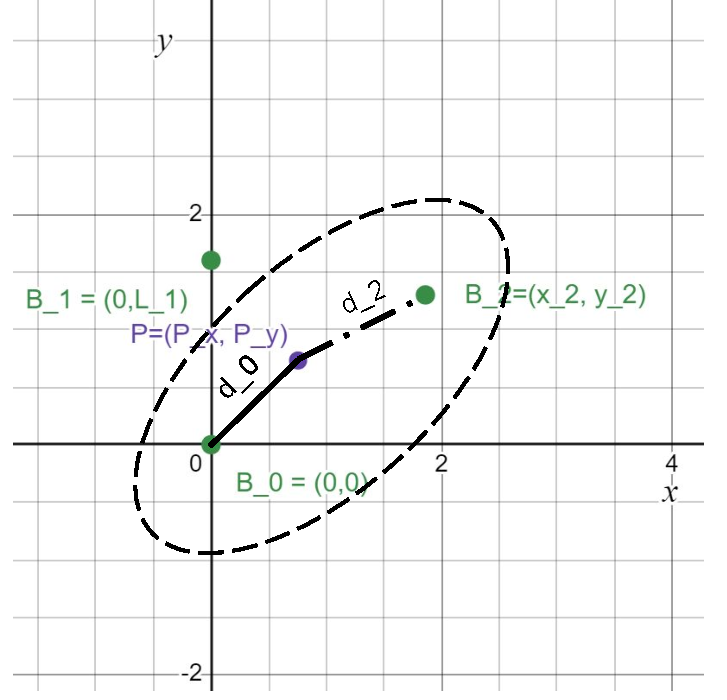
\includegraphics[width=\linewidth]{draw3.2.pdf}
~\label{fig:draw3_2}
    \end{minipage}
\end{figure} 
\FloatBarrier{}
Again here two cases must be considered:\\
\textbf{Case 1: $k_2>1$}\\
When the equation for $C_1$ was found, it was noted that the circle is distance $S_{c1}=\frac{-L_1}{k_1-1}$ units from $B_0$. Let $C_2$ be the circle made up of positions that $P$ could be at, considering only the ratio $k_2$. 
Since, the same procedure as the one used to find $C_1$ is used, we know that the the center of $C_2$ is $S_{c2}=\frac{-L_2}{k_2-2}$, where $L_2$ is the distance between $B_0$ and $B_1$. This applies to the radius also: $R_2=\left(\frac{L_2}{k_1-1}\sqrt{k_1}\right)$
The center of $C_2$
also lies on the line $M_2$ that passes through the points $B_0$ and $B_2$. Since the position of $B_2$ is known to be $(x_2,y_2)$, and $B_0$ is at $(0,0)$:
\begin{equation*}
    M_2: y=\frac{y_2}{x_2}x
\end{equation*}
\\\\
Let the center of $C_2$ be denoted as $(x_{c2},y_{c2})$. Since this point lies on the line $M_2$, we know that $y_{c2}=\frac{y_2}{x_2}x_{c2}$.
Additionally, using Pythagoras theorem, we have:
\begin{equation*}
    \begin{split}
        &x_{c2}^2 + y_{c2}^2 = S_{c2}^2\\
        &y_{c2} = \sqrt{ S_{c2}^2 - x_{c2}^2}\\
        &y_{c2} = \sqrt{\left(\frac{-L_2}{k_2-2}\right) - x_{c2}^2}\\
    \end{split}
\end{equation*}

This gives a system of equations with two variables:
\begin{equation}
    \begin{cases}
        y_{c2}=\frac{y_2}{x_2}x_{c2}\\ 
        y_{c2} = \sqrt{\left(\frac{-L_2}{k_2-2}\right) - x_{c2}^2}
    \end{cases}
\label{eq:system}
\end{equation}
\FloatBarrier{}
The~\textit{equations~\ref{eq:system}}, can be solved to find the center of $C_2$.
\begin{equation*}
    \begin{split}
        &\left(\frac{y_2}{x_2}\right)^2x_{c2} = \sqrt{\left(\frac{-L_2}{k_2-1}\right)^2 - x_{c2}^2}\\\\
        &\left(\frac{y_2}{x_2}\right)^2x_{c2}^2 = \left(\frac{-L_2}{k_2-1}\right)^2 - x_{c2}^2\\\\
        &x_{c2}^2\left(\left(\frac{y_2}{x_2}\right)^2+1\right) = \left(\frac{-L_2}{k_2-1}\right)^2\\\\
        &x_{c2} = \frac{-L_1}{k_1-1}\sqrt{\frac{1}{\left(\frac{y_2}{x_2}\right)^2+1}}\\\\
    \end{split}
\end{equation*}

Hence,
\begin{equation*}
    \begin{split}
        &y_{c2}=\frac{y_2}{x_2}\cdot x_{c2}\\
        &y_{c2}=\frac{y_2}{x_2}\cdot \frac{-L_1}{k_1-1}\sqrt{\frac{1}{\left(\frac{y_2}{x_2}\right)^2+1}}
    \end{split}
\end{equation*}
This gives the final question for the circle:
\begin{equation*}
    C_2: \left(x-\frac{-L_1}{k_1-1}\sqrt{\frac{1}{\left(\frac{y_2}{x_2}\right)^2+1}}\right)^2 + \left(y-\frac{y_2}{x_2}\cdot \frac{-L_1}{k_1-1}\sqrt{\frac{1}{\left(\frac{y_2}{x_2}\right)^2+1}}\right)^2= \left(\frac{L_2}{k_1-1}\sqrt{k_1}\right)^2
\end{equation*} 
\textbf{Case 2: $k_2=1$}\\
Just like \textbf{Case 2: $k_1=1$}, the possible positions of $P$ will also be on a line: $T_2$. This line will be perpendicular to $M_2$ and pass through the midpoint between $B_0$ and $B_1$.
\begin{equation*}
    \begin{split}
        &T_2: \left(y-\frac{y_2}{2} \right)= -\frac{x_2}{y_2}\left(x-\frac{x_2}{2} \right)\\
        &T_2: y=-\frac{x_{2}}{y_{2}}x+\frac{x_{2}^{2}+y_{2}^{2}}{2y_{2}}\\
        &T_2: y=-\frac{x_{2}}{y_{2}}x+\frac{L_2^2}{2y_{2}}\\
    \end{split}
\end{equation*}

\subsection{Finding the exact location of $P$}
Since, there are there are two cases for both $k_1$ and $k_2$, a total of 4 cases must be considered. \\
\textbf{Case 1: $k_1>1$ and $k_2>1$}\\
In this case, there are two circles formed $C_1$ and $C_2$. Since, the device $P$ lies on both circles, it must be one of the intersections between the two circles. The intersection(s) could be found by system of equations of the two circles.
But, this leads to the system of equation would be a quadratic in some cases as there would be two intersection points and would make find the solutions of this quadratic relatively difficult. 
\\
A simpler solution is using the cosine rule. Let's consider $\vec{R_{1p}}$, $\vec{R_{2p}}$ and $\vec{R_D}$
\begin{itemize}
    \item $\vec{R_{1p}}$ is the vector of magnitude $R_1$, and direction from the center of $C_1$ to $P$.
    \item $\vec{R_{2p}}$ is the vector of magnitude $R_2$, and direction from the center of $C_2$ to $P$. 
    \item $\vec{R_D}$ is the vector of magnitude $\sqrt{(0-x_c)^2 + \left(\frac{-L_1}{k_1-1}-y_c\right)^2}$, and direction from the center of $C_1$ to $C_2$
    \begin{equation*}
        \vec{R_D}=
        \begin{pmatrix}
            -x_c \\ 
            \frac{-L_1}{k_1-1}-y_c\\
        \end{pmatrix}
    \end{equation*}
\end{itemize}

The three vectors form a triangle. Let $\alpha$ be the angle between $\vec{R_D}$ and $\vec{R_{1p}}$. Let $\theta$ be the angle between $\vec{R_{1p}}$ and the x-axis. Therefore,
$\alpha + \theta = \pi + \arctan\left(\frac{\frac{-L_1}{k_1-1}-y_c}{-x_c}\right)$.
\\\\
Then using the cosine rule, $\alpha$ can be calculated.
\begin{equation*}
    \begin{split}
        R_2^2 & = R_1^2 + |\vec{R_D}|^2 - 2\cdot R_1^2\cdot|\vec{R_D}|^2\cos(\alpha)\\\\
        \alpha & = \arccos{\left(\frac{R_2^2 -R_1^2 - |\vec{R_D}|^2 }{- 2\cdot R_1^2\cdot|\vec{R_D}|^2}\right)}
    \end{split}
\end{equation*}
Then $\theta$ is calculated using:
\begin{equation*}
    \theta = \pi + \arctan{\left(\frac{\frac{-L_1}{k_1-1}-y_c}{-x_c}\right)} - \alpha
\end{equation*}

Since, $\theta$ is the angle of the vector $\vec{R_1}$, and has a starting position at $\left(0,\frac{-L_1}{k_1-1}\right)$, the coordinates of $P$ are:
\begin{equation}
    P~(P_x, P_y) = \left(R_1\cos(\theta), R_1\sin(\theta)+\frac{-L_1}{k_1-1}\right)
\label{eq:case1}
\end{equation}
\\\\
\textbf{Case 2: $k_1=1$ and $k_2>1$ }
\\
In this case, and intesection between a line and a circle is used. Since $k_1=1$ and $k_2>1$ the phone $P$ lies on the line $T_1$ and on the circle $C_2$. Since p
This gives a system of equations:
\begin{equation}
    \begin{cases}
        P_y=\frac{L_1}{2} \\ 
        (P_x-x_{c2})^2 + (P_y-y_{c2})^2 = R_2^2\\
    \end{cases}
\label{eq:system2}
\end{equation}
Which can be simplified into:
\begin{equation*}
    \begin{cases}
        P_y=\frac{L_1}{2} \\ 
        P_x = \sqrt{R_2^2 - (P_y-y_{c2})^2} + x_{c2}\\
    \end{cases}
\end{equation*}
And solving this equation gives the value for $P_x=  \sqrt{R_2^2 - \left(\frac{L_1}{2}-y_{c2}\right)^2} + x_{c2}$
\begin{equation}
    P~(P_x, P_y) = \left(\sqrt{R_2^2 - \left(\frac{L_1}{2}-y_{c2}\right)^2} + x_{c2},~\frac{L_1}{2}\right)
\label{eq:case2}
\end{equation}
\\\\
\textbf{Case 3: $k_1>1$ and $k_2=1$ }
\\
In this case, also an intersection between the line $T_2$ and the circle $C_1$ is to be found. 
\begin{equation*}
    \begin{cases}
        P_y=-\frac{x_{2}}{y_{2}}P_x+\frac{L_2^2}{2y_{2}}\\ 
        P_x^2 + \left(P_y - \frac{-L_1}{k_1-1}\right)R_1^2\\
    \end{cases}
\end{equation*}
Substituing $P_y$ in the equation of $C_1$ with $-\frac{x_{2}}{y_{2}}P_x+\frac{L_2^2}{2y_{2}}$, gives:
\begin{equation*}
    P_x^2 + \left(\frac{-x_2}{y_2}P_x + \frac{L_2^2}{2y_2} - \frac{L_1}{k_1-1}\right)^2 = R_1^2
\end{equation*}
Let: $a=\frac{-x_2}{y_2}$, $b=\frac{L_2^2}{2y_2}$ and $c=\frac{L_1}{k_1-1}$
\begin{equation*}
    \begin{split}
      &P_x^2 + \left(aP_x + b - c\right)^2 = R_1^2\\
      &P_x=\frac{-2a(b-c) \pm \sqrt{(2ab-2ac)^2 -4(1+a^2)((b-c)^2-R_1^2)}}{2(1+a^2)}\\
    \end{split}
\end{equation*}
Hence, solving this system gives the position of $P$ to be:
\begin{equation}
    P~(P_x, P_y)=\left(P_x,\frac{x_{2}}{y_{2}}P_x+\frac{L_2^2}{2y_{2}}\right)
\label{eq:case3}
\end{equation}
The whole equation isn't displayed due to it being lengthy and unable to fit into one page. 
\\\\
\textbf{Case 4: $k_1=1$ and $k_2=1$ }
\\
In this case, it is an intersection between $T_1$ and $T_2$:
\begin{equation*}
    \begin{cases}
        P_y = \frac{L_1}{2}\\
        P_y=-\frac{x_{2}}{y_{2}}P_x+\frac{L_2^2}{2y_{2}}\\ 
    \end{cases}
\end{equation*}
Solving this system of equations gives:
\begin{equation*}
    \begin{split}
        &\frac{L_1}{2}=-\frac{x_{2}}{y_{2}}P_x+\frac{L_2^2}{2y_{2}}\\\\
        &P_x = \left(\frac{L_1}{2}-\frac{L_2^2}{2y_{2}}\right)\cdot \frac{-y_{2}}{x_{2}}\\
    \end{split}
\end{equation*}
\begin{equation}
    P~(P_x, P_y)=\left(\left(\frac{L_1}{2}-\frac{L_2^2}{2y_{2}}\right)\cdot \frac{-y_{2}}{x_{2}},~\frac{L_1}{2}\right)
\label{eq:case4}
\end{equation}

\section{Generalized Formula for Location of $P$}

Using the given knowns:
\begin{itemize}
    \item $k_1$: Ratio of Intensities received from $B_0$ and $B_1$
    \item $k_2$: Ratio of Intensities received from $B_0$ and $B_2$
    \item $B_0$: Location of Receiver 0 at $(0,0)$
    \item $B_1$: Location of Receiver 1 at $(0,L)$
    \item $B_2$: Location of Receiver 2 at $(x_2,y_2)$ for $x_2,y_2\in \mathbb{R}$
    \item $L_1$: Distance between $B_0$ and $B_1$
    \item $L_2$: Distance between $B_0$ and $B_2$
    \item $x_{c2}$: $\frac{-L_1}{k_1-1}\sqrt{\frac{1}{\left(\frac{y_2}{x_2}\right)^2+1}}$
    \item $y_{c2}$: $\frac{y_2}{x_2}\cdot\frac{-L_1}{k_1-1}\sqrt{\frac{1}{\left(\frac{y_2}{x_2}\right)^2+1}}$
\end{itemize}
$P$ is located at $(P_x, P_y$)
\begin{equation*}
    P_x=
    \begin{cases}
        P_x~from~equation~\ref{eq:case1},~if~k_1>1~and~k_2>1\\
        P_x~from~equation~\ref{eq:case2},~if~k_1>=1and~k_2>1\\ 
        P_x~from~equation~\ref{eq:case3},~if~k_1>1~and~k_2=1\\
        P_x~from~equation~\ref{eq:case4},~if~k_1=~and~k_2=1\\
    \end{cases}
\end{equation*}

\begin{equation*}
    P_y=
    \begin{cases}
        P_y~from~equation~\ref{eq:case1},~if~k_1>1~and~k_2>1\\
        P_y~from~equation~\ref{eq:case2},~if~k_1>=1and~k_2>1\\ 
        P_y~from~equation~\ref{eq:case3},~if~k_1>1~and~k_2=1\\
        P_y~from~equation~\ref{eq:case4},~if~k_1=~and~k_2=1\\
    \end{cases}
\end{equation*}

\section{Conclusion }
Using the location of 3 Base stations, and the ratio of intensities received by them by a lost electromagnetic wave emmiting device can be found using an equation for different conditions of the intensities. 
The location of this EM device is relative to the the base station $B_0$ and is found using intersection of 2 circles, a circle and line or 2 lines, depending on the conditions of the ratio of intensities.

\subsection{Evaluation}
The model created works only in a 2 dimensional system. Such systems could be implemented for cities or even small countries that don't have drastic altitude changes. Althought this model find the exact location 
of $P$, in real life, certain limitations such as measurement uncertainty which propagates as one intensity is divided by the other (such as $\frac{I_0}{I_1}$).

This model could be expanded into a 3 dimensional system, however, during my research for this exploration it was found that GPS devices apply a much simpler and different approach. A GPS system consists of 4 satellites placed in 3D space,
that send a signal to the lost device, with a time stamp. The distance between the device and each of the satellites is determined using the equation $c=\frac{D}{\Delta t}$, where $\Delta t$ is the time taken for the signal to reach the device, $c\approx 3\cdot 10^8 m/s$ is the speed of electromagnetic waves and $D$ is the distance.
After finding the 4 Distances, they are used to draw spheres centered at each satellites and of radius with their corresponding distance. The intersection of the 4 spheres is where the lost device is located.

Albeit, this positioning system not working on a global scale, this could work on local scales. Devices such as apple air tags, that use nearby apple devices to transmit their location could be utilizing this methodology of positioning.

\printbibliography



\end{document}
